\def\sphoyear{2021}
\setcounter{section}{0}
% Headers and Descriptions
\fancyhead[L]{\textbf{SPhO \sphoyear}} \fancyhead[R]{\textbf{Questions}}


\begin{titlepage}
\centering

{\Huge\bfseries SPhO \sphoyear}

\vspace{1cm}

{\LARGE Problem Set}

\vspace{2cm}

{\Large Compiled by: Tan Chien Hao, \texttt{www.tchlabs.net}}

\vspace{2cm}

{\Large Edited/Proofread by: Keith Chan, Sun Yu Chieh}
%Collaborators please feel free to add on!

\vspace{2cm}

{\large Suggest changes at: \github}


\vfill

{\itshape Last edited: \today}
\end{titlepage}

\begin{problem}
    A parallel-plate capacitor is shown in the diagram with plate area of $A = \qty{10.5}{\cm}^2$ and plate separation $2d = \qty{7.12}{mm}$. The left half of the gap is filled with material of dielectric constant $\kappa_1 = 21.0$; the top of the right half is filled with material of dielectric constant $\kappa_2 = 42.0$; the bottom of the right half is filled with material of dielectric constant $\kappa_3 = 58.0$. What is the capacitance? \hfill $[4]$
    \begin{figure}[H]
        \centering
        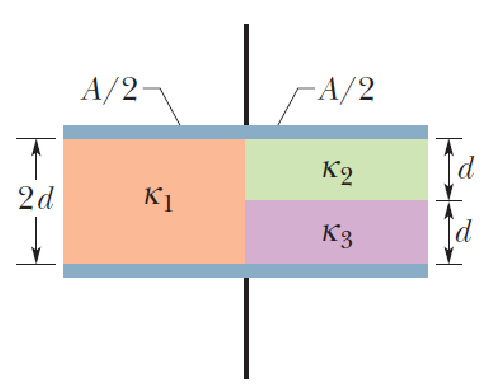
\includegraphics[width=0.5\textwidth]{spho_book_TYS_images/2021SPhO_1.png}
        \label{fig:1}
    \end{figure}
\end{problem}

\begin{problem}
    In the rectangle shown, the sides have lengths \qty{5.0}{\cm} and \qty{15}{\cm}, $q1 = \qty{-5.0}{\micro\C}$, and $q2 = \qty{+2.0}{\micro\C}$. 
    \begin{figure}[H]
        \centering
        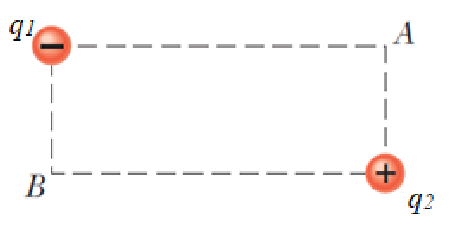
\includegraphics{spho_book_TYS_images/2021SPhO_2.png}
    \end{figure}  
    With  $V = 0$ at infinity, what is the electric potential at
    \begin{subproblemalph}
        \item corner A and \hfill $[1]$
        \item corner B? \hfill $[1]$
        \item How much work is required to move a charge $q3 = \qty{+3.0}{\micro\C}$ from B to A along a diagonal of the rectangle? \hfill $[1]$
        \item Does this work increase or decrease the electric potential energy of the three-charge system? \hfill $[1]$
    \end{subproblemalph}
    Is more, less, or the same work required if q3 is moved along a path that is
    \begin{subproblemalph}
        \setcounter{enumi}{4}
        \item inside the rectangle but not on a diagonal and \hfill $[0.5]$        
        \item outside the rectangle?  \hfill $[0.5]$
    \end{subproblemalph}
\end{problem}

\begin{problem}
    The conducting rod shown in the figure has length $L$ and is being pulled along horizontal, frictionless conducting rails at a constant velocity $\vec{v}$. The rails are connected at one end with a metal strip. A uniform magnetic field $\vec{B}$, directed out of the page, fills the region in which the rod moves. Assume that $L = 10 \unit{cm}$, $v = \qty{5.0}{\m\s^{-1}}$, and $B = \qty{1.2}{T}$. 
    \begin{figure}[H]
        \centering
        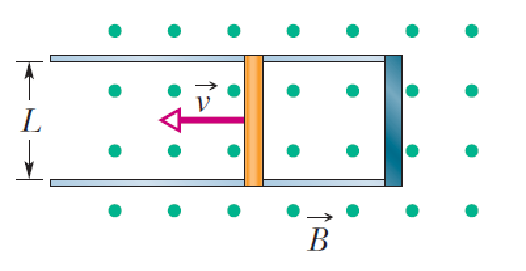
\includegraphics{spho_book_TYS_images/2021SPhO_3.png}
    \end{figure}
    What are the
    \begin{subproblemalph}
        \item magnitude and \hfill [1]
        \item direction (up or down the page) of the emf induced in the rod? \hfill [0.5]
        \item magnitude and \hfill [0.5]
        \item direction of the current in the conducting loop? \hfill [0.5]
    \end{subproblemalph}
    Assume that the resistance of the rod is $0.40 \Omega$ and that the resistance of the rails and metal strip is negligibly small.
    \begin{subproblemalph}
        \setcounter{enumi}{4}
        \item At what rate is thermal energy being generated in the rod? \hfill [1]
        \item What external force on the rod is needed to maintain $\vec{v}$? \hfill [1.5]
        \item At what rate does this force do work on the rod? \hfill [1]
    \end{subproblemalph}
\end{problem}
\newpage
\begin{problem}
    In the figure shown, after the switch S is closed at time $t = 0$, the emf of the source is automatically adjusted to maintain a constant current I through S.
    \begin{figure}[H]
        \centering
        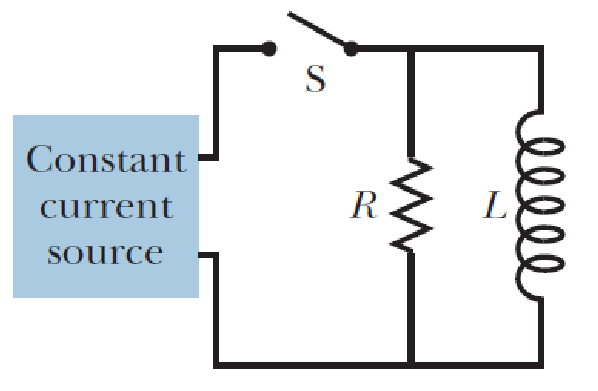
\includegraphics{spho_book_TYS_images/2021SPhO_4.png}
    \end{figure}
    \begin{subproblemalph}
        \item Find the current through the inductor as
a function of time. \hfill $[4]$
        \item At what time is the current through the
resistor equal to the current through the
inductor? \hfill $[1]$
    \end{subproblemalph} 
\end{problem}

\begin{problem}
    In the figure shown, a string, tied to a sinusoidal oscillator at P and running over a support at Q, is stretched by a block of mass m. The separation L between P and Q is \qty{1.20}{m}, and the frequency f of the oscillator is fixed at \qty{120}{Hz}. The amplitude of the motion at P is small enough for that point to be considered a node. A node also exists at Q. A standing wave appears when the mass of the hanging block is \qty{286.1}{g} or \qty{447.0}{g}, but not for any intermediate mass. What is the linear density of the string? \hfill $[6]$
    \begin{figure}[H]
        \centering
        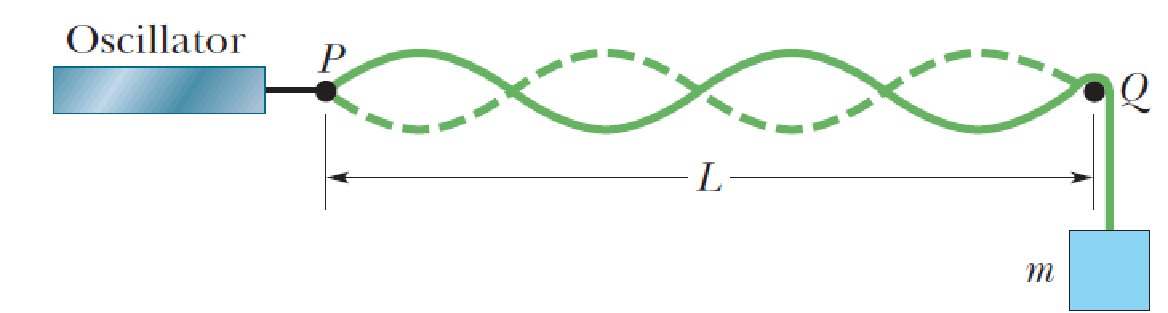
\includegraphics[width=0.8\linewidth]{spho_book_TYS_images/2021SPhO_5.png}
    \end{figure}
\end{problem}

\begin{problem}
    Calculate the minimum kinetic energy an electron must have in order to be constrained within the nucleus, with a typical nuclear radius of $r = \qty{6e-15}{\m}$. Assume that the uncertainty of this electron’s position is equal to the nuclear radius r. Treat the electron relativistically. \hfill $[6]$
\end{problem}
\newpage
\begin{problem}
    A small \qty{50}{g} block slides down a frictionless surface through height $h = \qty{20}{\cm}$ and then sticks to a uniform rod of mass \qty{100}{g} and length \qty{40}{cm}. The rod pivots about point O through angle $\theta$ before momentarily stopping. Find $\theta$. \hfill $[10]$
    \begin{figure}[H]
        \centering
        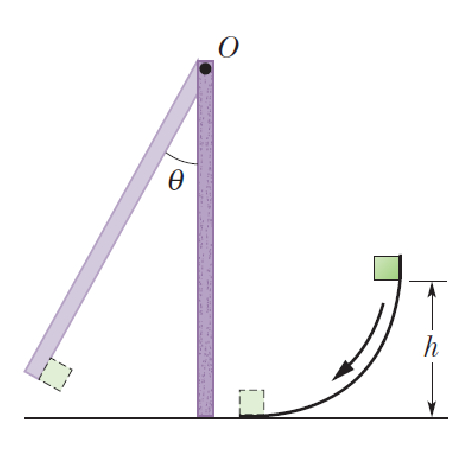
\includegraphics{spho_book_TYS_images/2021SPhO_7.png}
    \end{figure}
\end{problem}

\begin{problem}
    The figure shows a reversible cycle through which \qty{1.00}{mol} of a monatomic ideal gas is taken. Volume $V_c = 8.00V_b$. Process $bc$ is an adiabatic expansion, with $p_b = \qty{10.0}{atm}$ and $V_b = \qty{1.00e-3}{\m^3}$. 
    \begin{figure}[H]
        \centering
        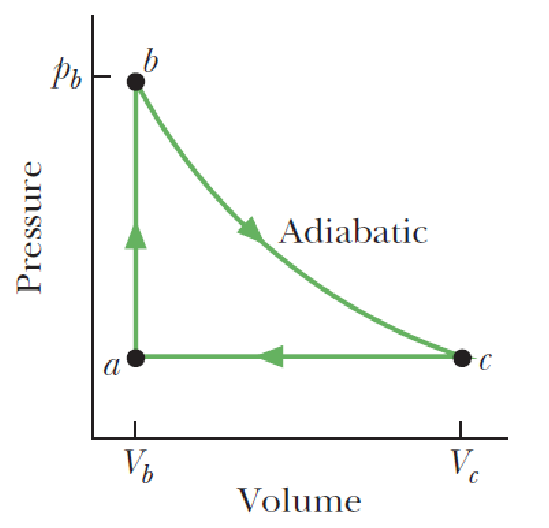
\includegraphics[width=0.5\textwidth]{spho_book_TYS_images/2021SPhO_8.png}
    \end{figure}
    
    For the cycle, find
    \begin{subproblemalph}
        \item the energy added to the gas as heat, \hfill $[3]$
        \item the energy leaving the gas as heat, \hfill $[3]$
        \item the net work done by the gas, and \hfill $[1]$
        \item the efficiency of the cycle. \hfill $[1]$
    \end{subproblemalph}
\end{problem}

\begin{problem}
    An ideal massless spring with spring constant $k = \qty{10}{\N \m^{-1}}$ and unstretched length $L = \qty{0.5}{\m}$ is attached to point O on axis of a disc. It has a point mass $m = \qty{1}{\kg}$ attached at $L_1 = \qty{0.2}{\m}$ of the unstretched spring. The spring is stretched and the other end is attached to point A on the edge of the disc at $R_0 = \qty{1}{\m}$. The point mass is constrained to move radially only.
    \begin{figure}[H]
        \centering
        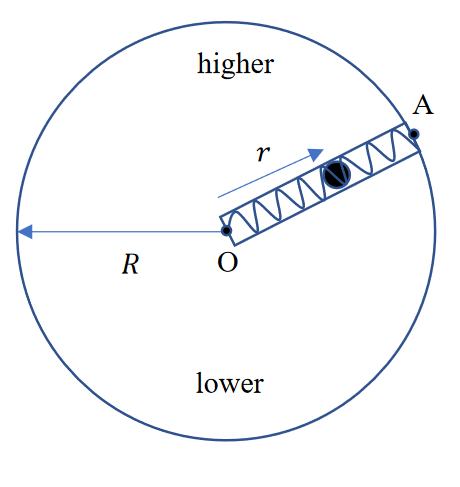
\includegraphics{spho_book_TYS_images/2021SPhO_9.png}
    \end{figure}
    The disc can rotate around the axis at a constant an angular frequency $\omega$. Take $t = \qty{0}{\s}$ when OA is horizontal and A is to the right and the disc is rotating anti-clockwise. Although some air resistance will help the system achieve a steady state, you may assume that air resistance is negligible in your working.
    \begin{subproblemalph}
        \item If the disc is \textbf{horizontal} and $\omega = 0$, derive an expression for the effective spring constant $k_t$ in terms of the given parameters. \hfill $[5]$
        \item If the disc is horizontal and rotating and constant angular velocity $\omega$, derive an expression for $r_0$, the equilibrium position of the mass. \hfill $[5]$
        \item If the disc is at an angle $\varphi = \qty{0.4}{rad}$ from the horizontal, what is the lowest angular frequency $\omega$ where the point mass can just about reach the edge of the disc at a steady state? \hfill $[5]$
    \end{subproblemalph}
\end{problem}
\newpage
\begin{problem}
    Consider Young’s double slit experiment as shown in the below figure (a). Monochromatic light is being used. Further assume that the screen distance $l$ is much larger than the slit separation $d$ (Figure (b))
    \begin{figure}
        \centering
        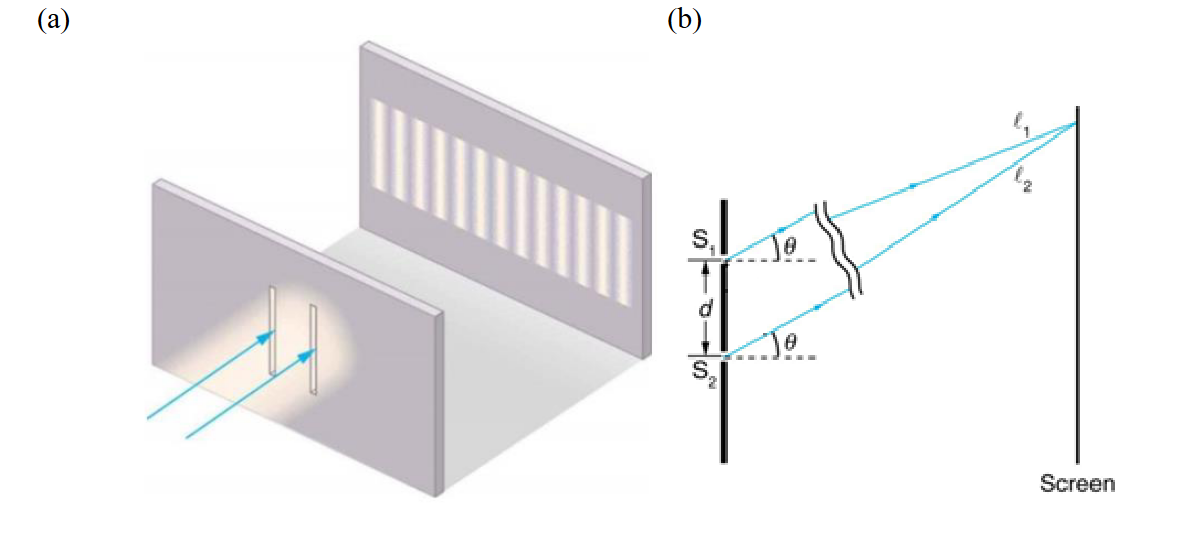
\includegraphics[width = 0.8\textwidth]{spho_book_TYS_images/2021SPhO_10.png}
    \end{figure}
    \begin{subproblemalph}
        \item Under what condition does Young’s experiment show interference pattern? \hfill $[0.5]$
        \item Determine the conditions for obtaining constructive and destructive interference. \hfill $[2]$
        \item Determine the distance $\Delta y$ between adjacent fringes (maxima), assuming that $\theta$ (Figure (b)) \hfill $[2]$
is small.
        \item Determine the intensity $I$ of the diffraction pattern’s maxima. You may use \[\sin\alpha + \sin\beta = 2 \cos\frac{1}{2}\left(\alpha-\beta\right)\sin\frac{1}{2}\left(\alpha+\beta\right)\] \hfill $[4.5]$
    \end{subproblemalph}
\end{problem}